\documentclass["WS\space 16-17\space -\space LaTeX-Kurs\space -\space Praesentation\space -\space 1.tex"]{subfiles}

\begin{document}

%kein WYSIWYG
%	"Programmieren" / Funktionsweise / Übersetzen
%	
%	Screenshots:
%		0. Dokument öffnen
%		1. Editor / PDF
%		2. Kompilierbutton
%		3. Schreiben zwischen begin und end Document
%
%	(Temporäre / Hilfsdateien)
\section{Editor}
\begin{frame}[c]
	\begin{center}
		\LARGE \textbf{Editor}
	\end{center}
\end{frame}


\begin{frame}[c]{Kompilieren in TeXstudio}
	\begin{figure}[htbp]
\centering
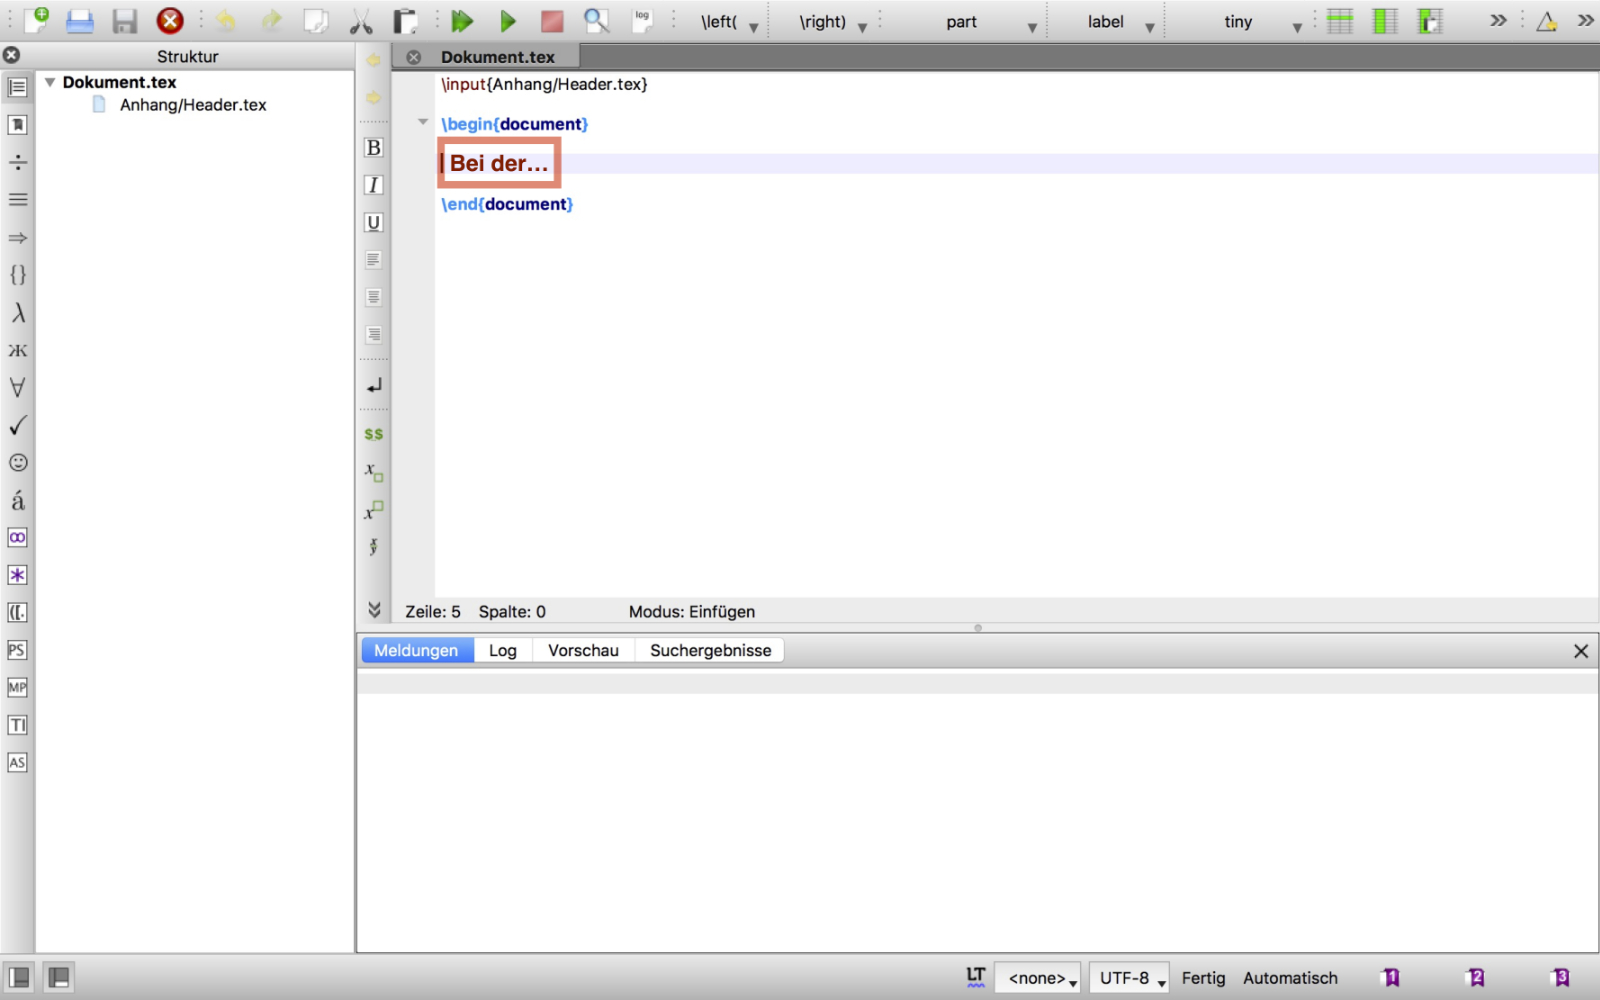
\includegraphics[width=0.9\textwidth]{img/editor/1.jpg}
%\caption{My Nice Figure.}
\end{figure}
\end{frame}


\begin{frame}[c]{Kompilieren in TeXstudio}
	\begin{figure}[htbp]
\centering
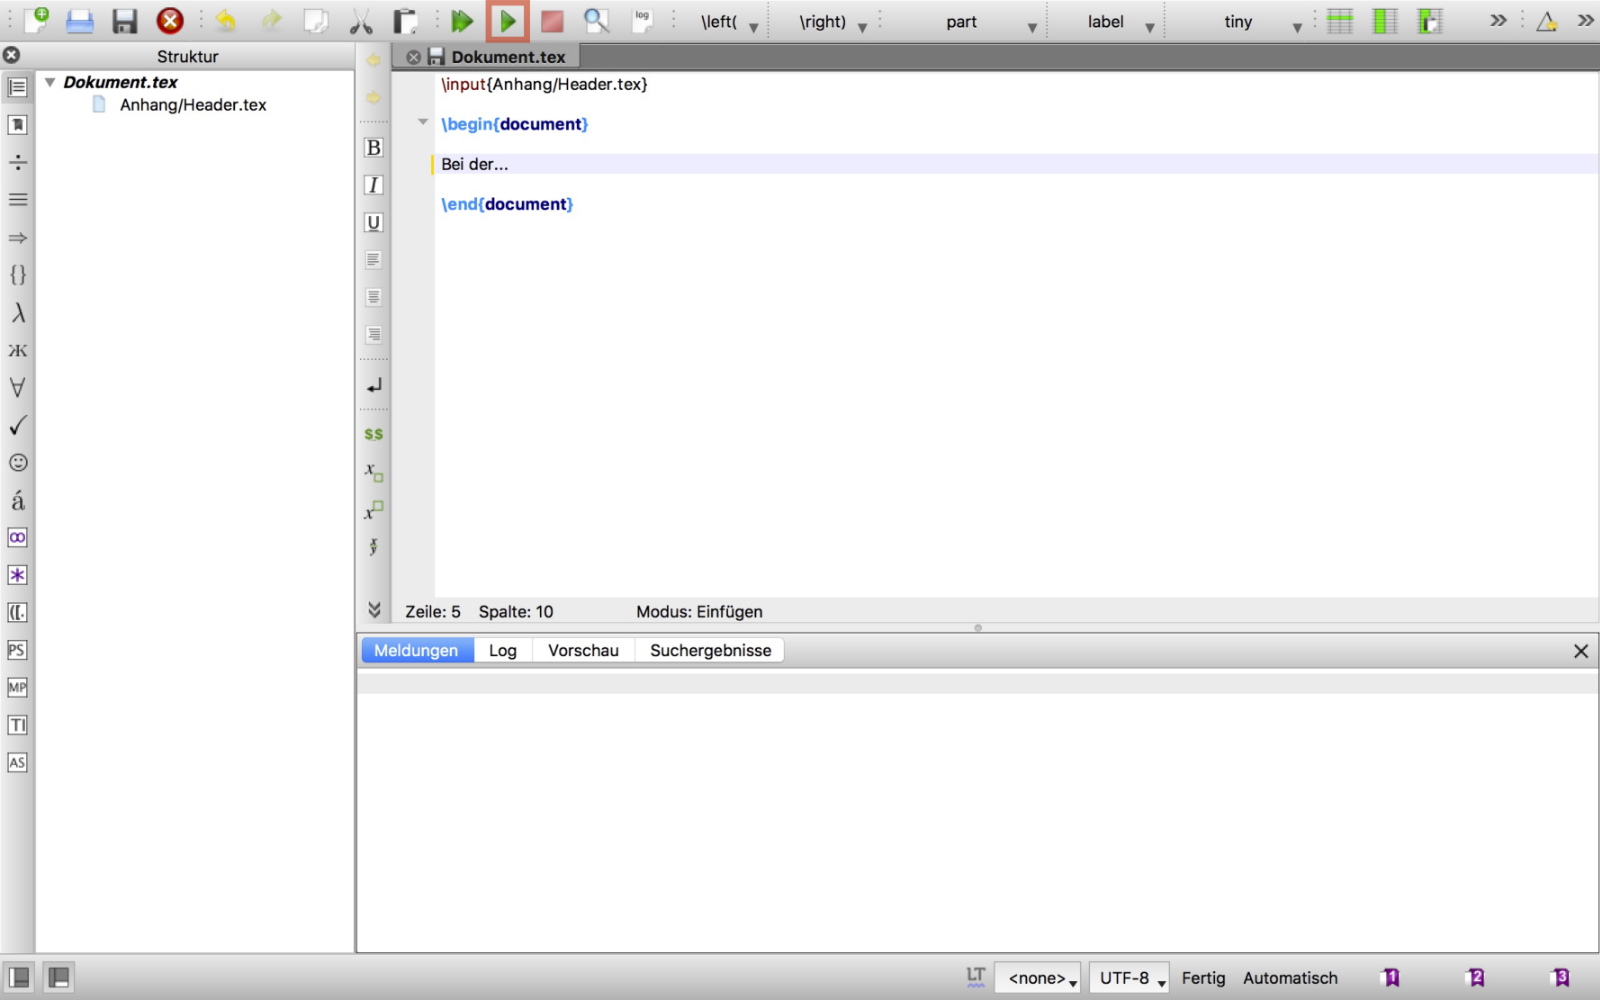
\includegraphics[width=0.9\textwidth]{img/editor/2.jpg}
%\caption{My Nice Figure.}
\end{figure}
\end{frame}

\begin{frame}[c]{Kompilieren in TeXstudio}
	\begin{figure}[htbp]
\centering
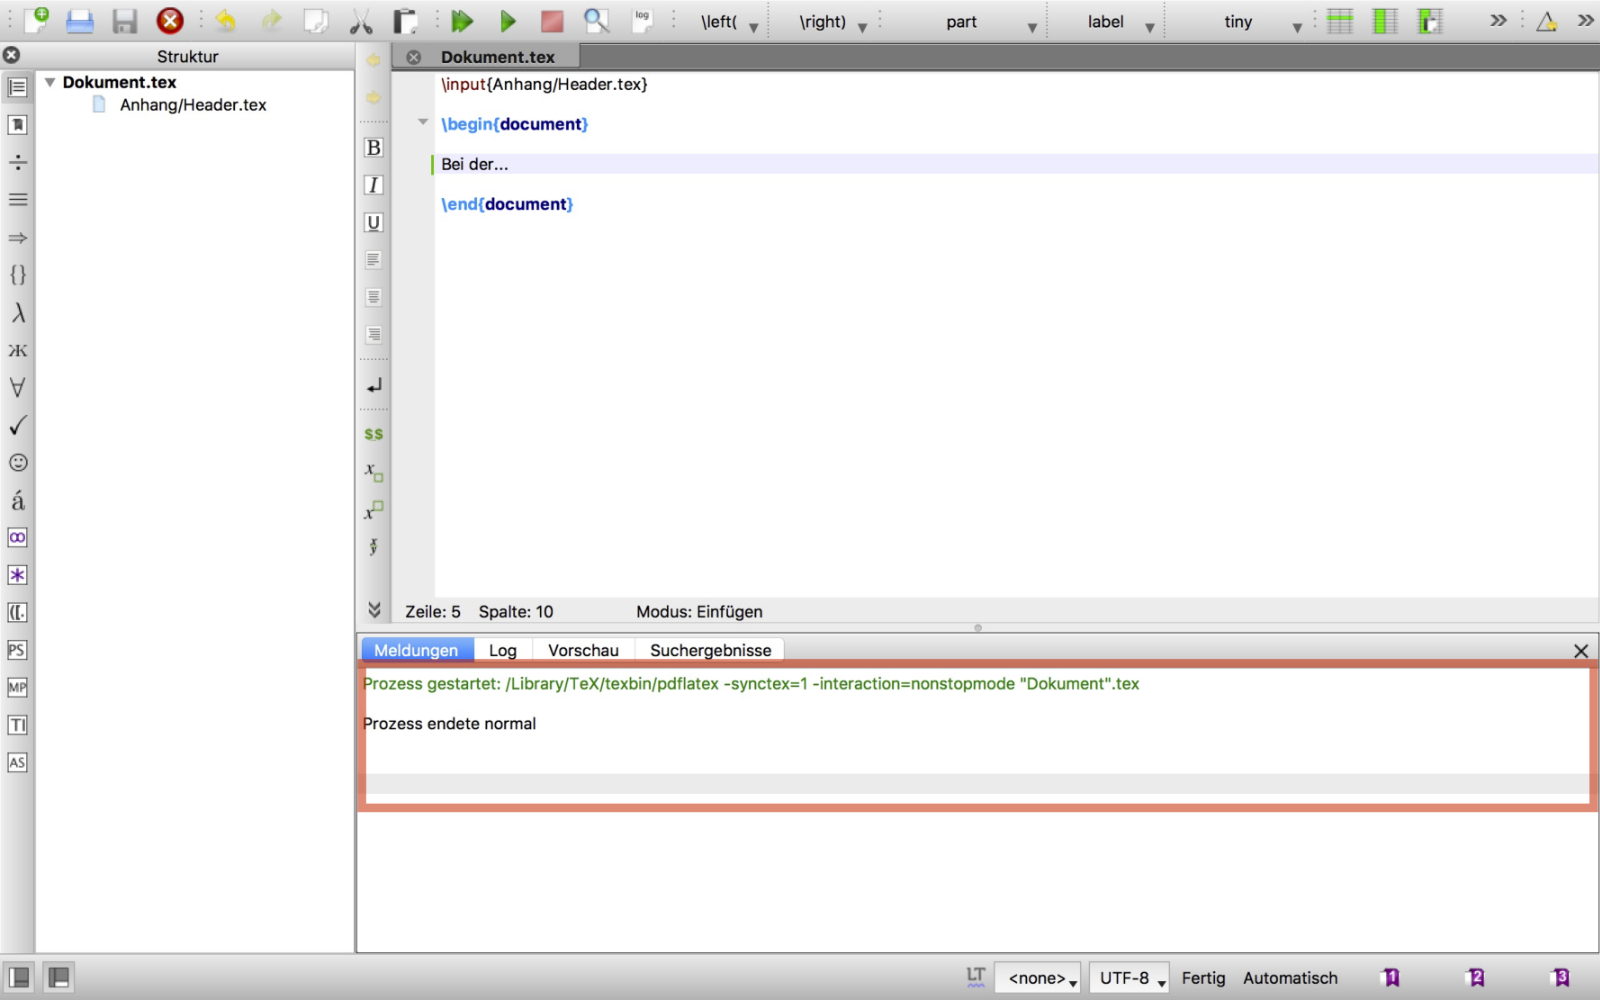
\includegraphics[width=0.9\textwidth]{img/editor/3.jpg}
%\caption{My Nice Figure.}
\end{figure}
\end{frame}

\begin{frame}[c]{Kompilieren in TeXstudio}
	\begin{figure}[htbp]
\centering
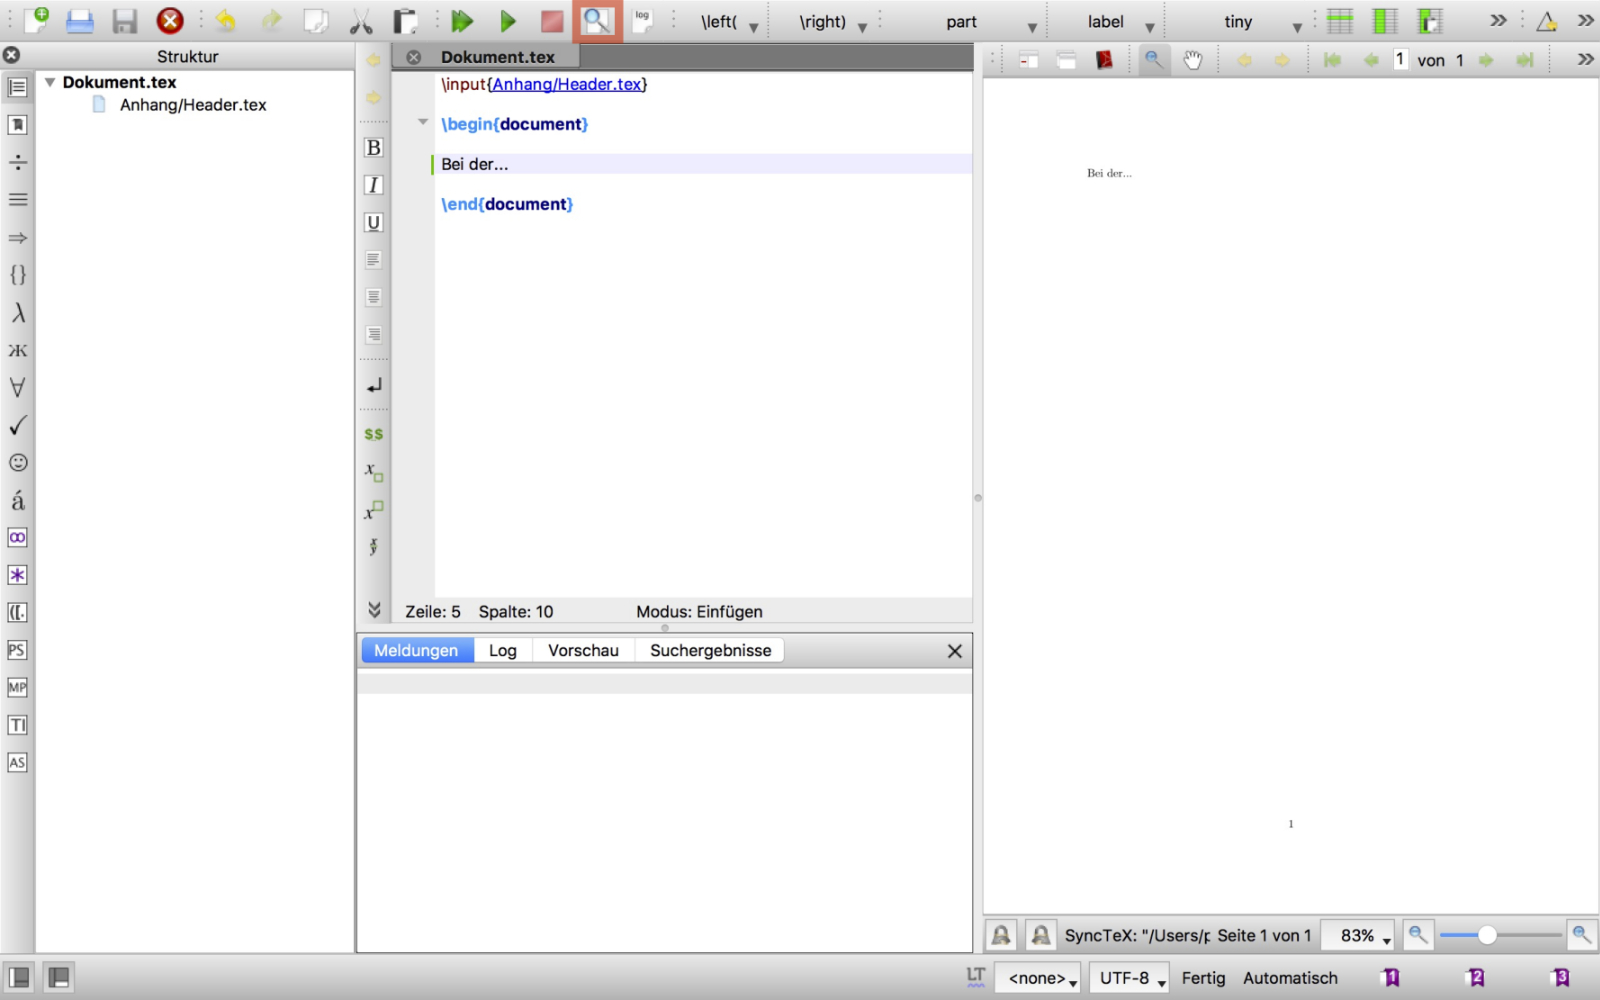
\includegraphics[width=0.9\textwidth]{img/editor/4.jpg}
%\caption{My Nice Figure.}
\end{figure}
\end{frame}

\begin{frame}[c]{Windows/Linux-Tastatur}
	\begin{figure}[htbp]
\centering
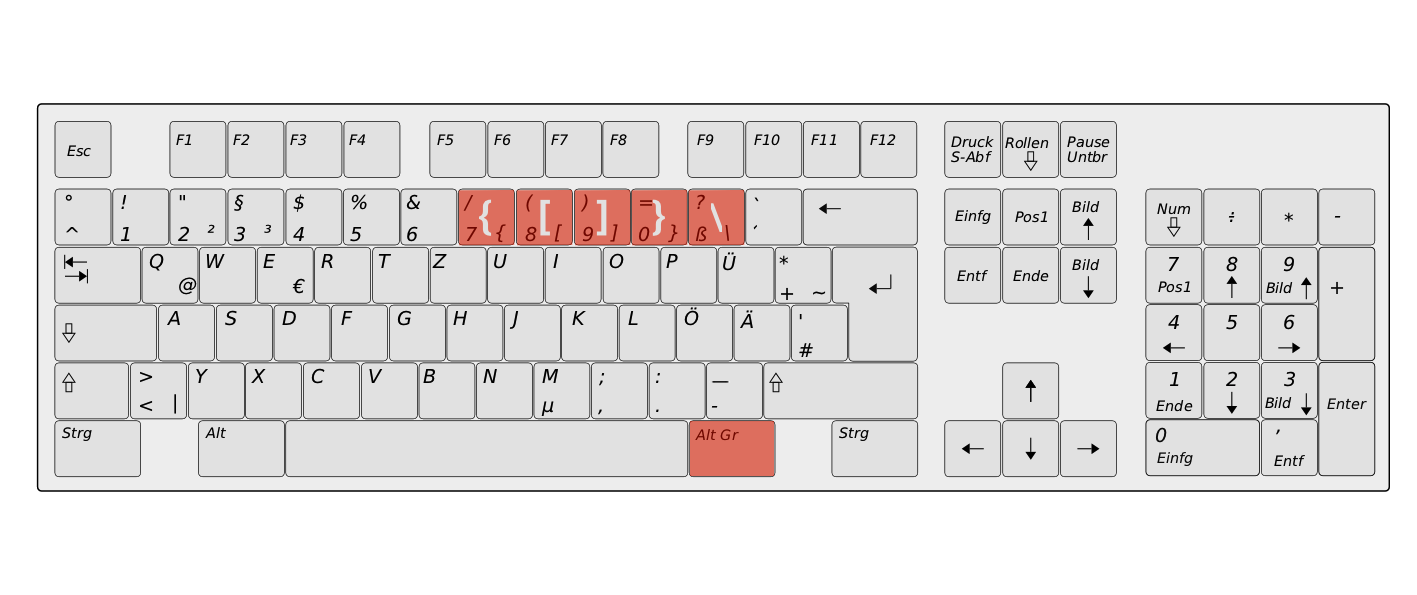
\includegraphics[width=1.0\textwidth]{img/tastatur/tastatur_win.png}
%\caption{My Nice Figure.}
\end{figure}
\end{frame}

\begin{frame}[c]{Mac-Tastatur}
	\begin{figure}[htbp]
\centering
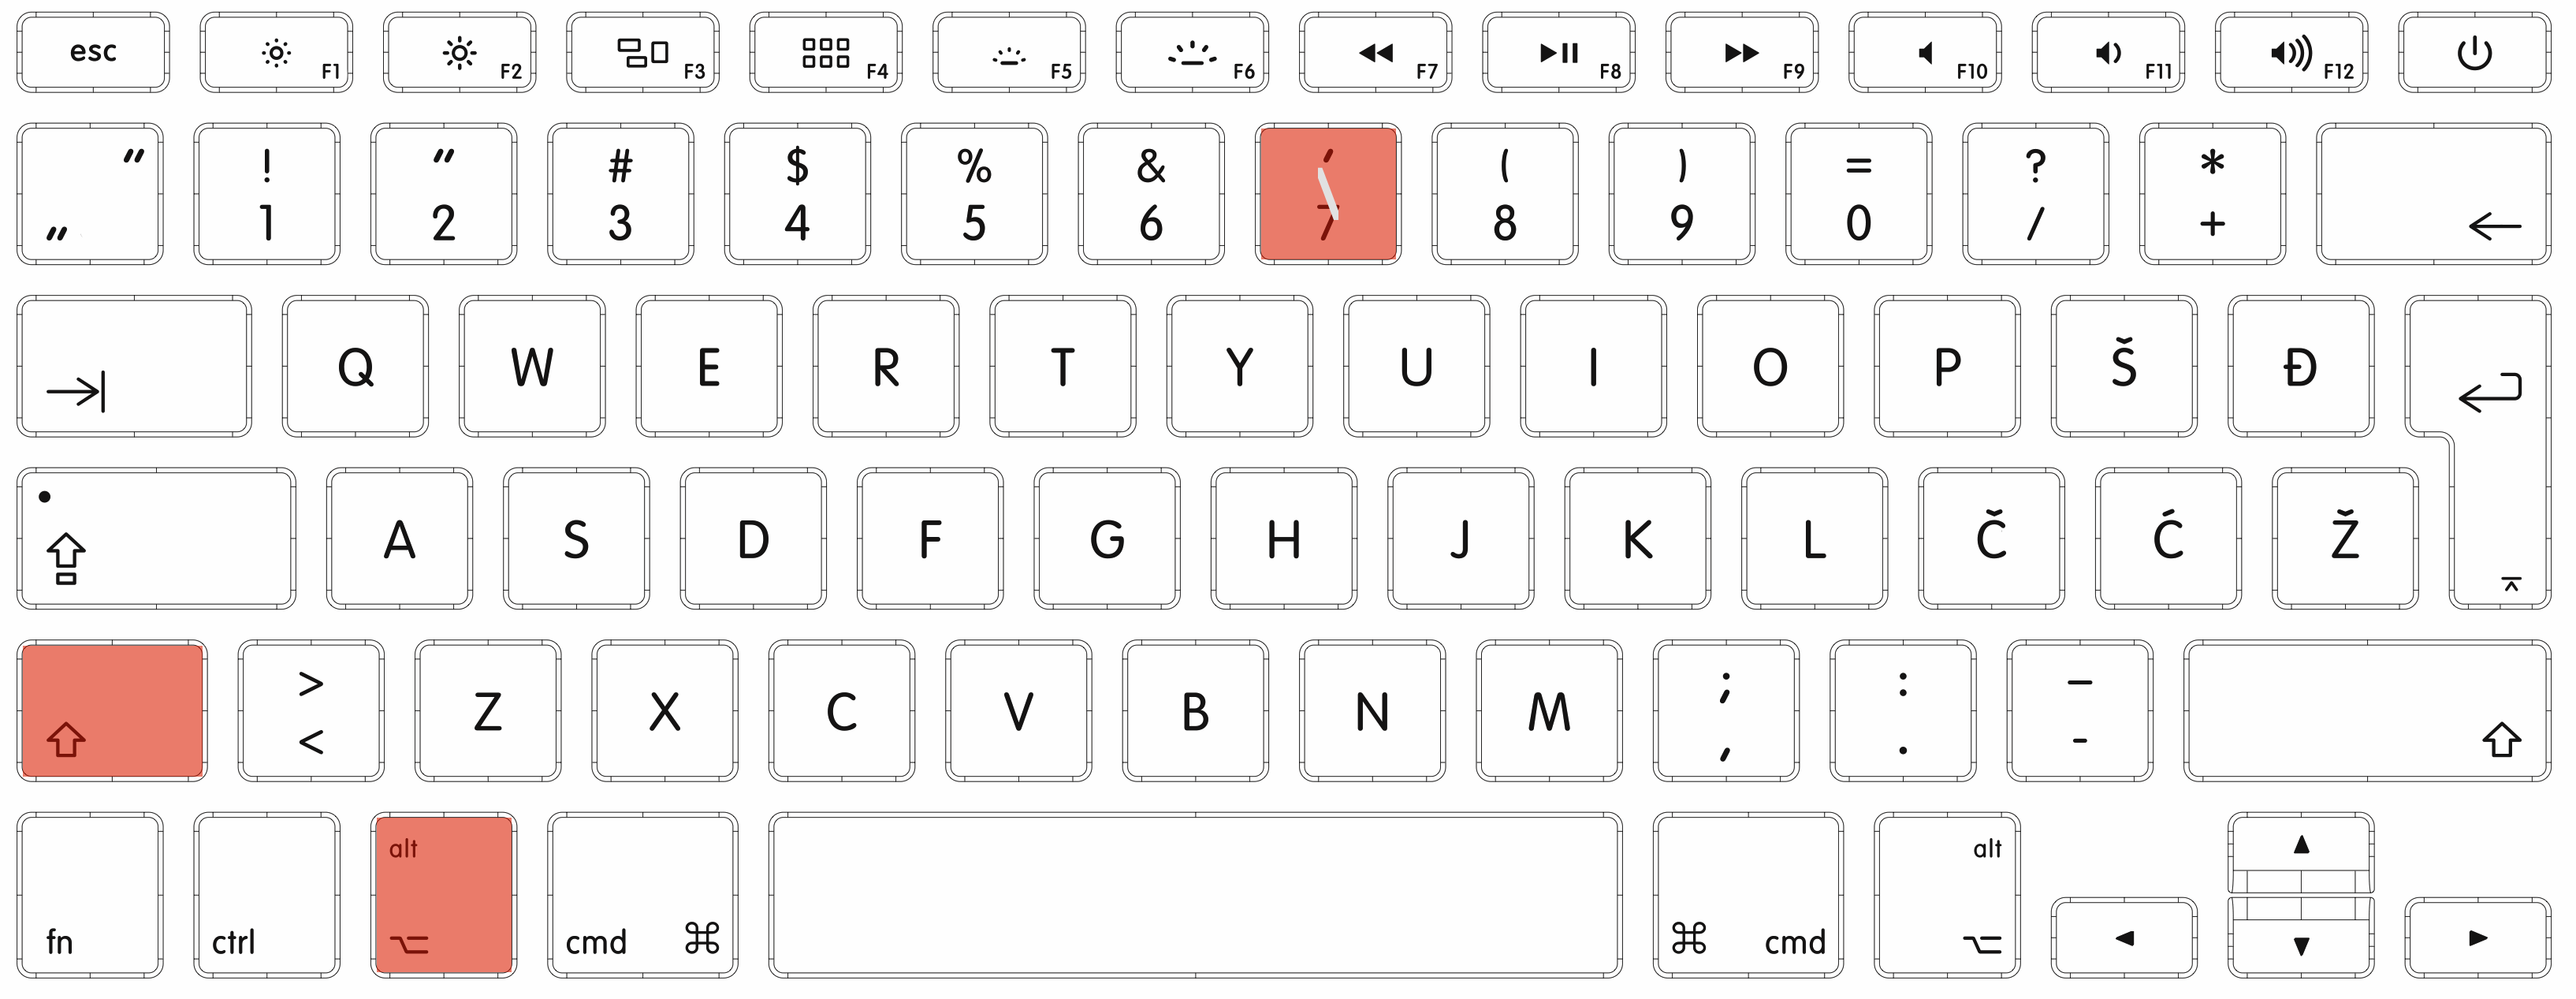
\includegraphics[width=1.0\textwidth]{img/tastatur/tastatur_mac_shift.png}
%\caption{My Nice Figure.}
\end{figure}
\end{frame}


\begin{frame}[c]{Mac-Tastatur}
	\begin{figure}[htbp]
\centering
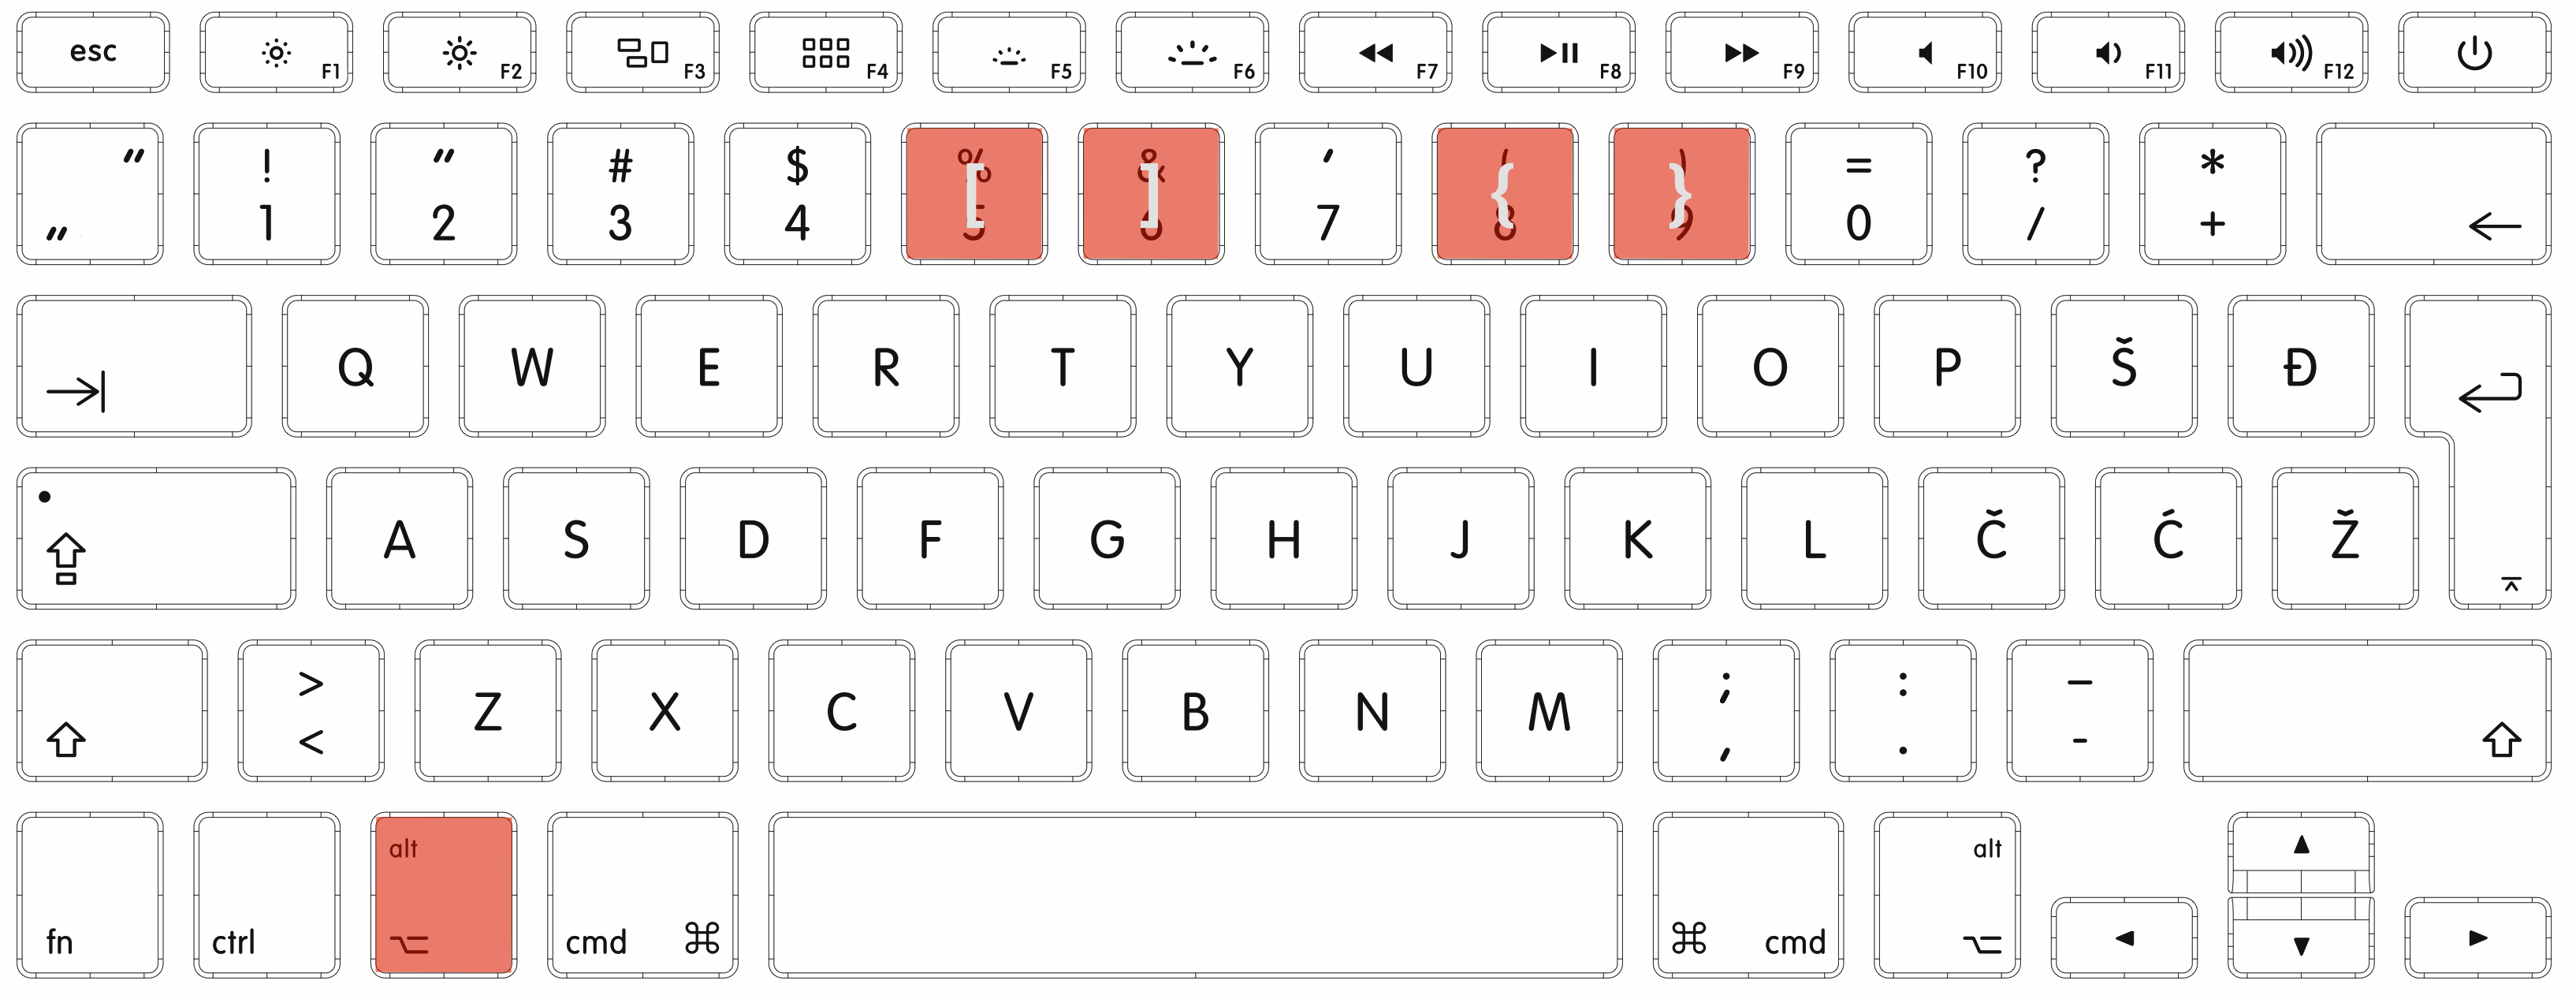
\includegraphics[width=1.0\textwidth]{img/tastatur/tastatur_mac_alt.png}
%\caption{My Nice Figure.}
\end{figure}
\end{frame}



\end{document}